\documentclass{llncs}


\usepackage{graphicx}
\usepackage[hidelinks]{hyperref}
\usepackage[nameinlink]{cleveref}
%obrázky, hyperlink, hyperlink s menom

\begin{document}
\sloppy
%text nepreteká do okrajov

\title{Utilization of Exercise Difficulty Rating by Students for Recommendation}
\titlerunning{}
\author{Martin Labaj, M\'{a}ria Bielikov\'{a}}
\authorrunning{}
\institute{Slovak University of Technology in Bratislava,\\ Faculty of Informatics and Information Technologies,\\
Ilkovi\v{c}ova 2, 842 16 Bratislava, Slovakia\\
\email{\{martin.labaj, maria.bielikova\}@stuba.sk}}

\maketitle

%abstrakt
\begin{abstract}
Recommendation plays a vital role in adaptive educational systems. Learners often face large body of educational materials including not only texts (explanations), but also interactive content such as exercises and questions. These require various knowledge levels of multiple topics. For effective learning, personalized recommendation of the most appropriate items according to the learner's current knowledge level and preferences is an essential feature. In this paper, we describe a learning object recommendation method based on students’ explicit difficulty ratings during and after exercise/question solving. It is based on comparing the learner’s state when the recommendation is to be made against his peers with similar knowledge in the moment when they rated the difficulty. To deal with sparsity of ratings that are even further filtered, we also propose two solutions to either adaptively elicit ratings in appropriate moments during learners work, or to predict ratings from implicit user actions. We evaluate the method in ALEF \textendash~adaptive web-based educational system.

\keywords{learning object difficulty, exercise difficulty rating, personalized recommendation, rating prediction, learning network}
\end{abstract}

\section{Introduction and related work}
\label{sec1}

Nowadays educational systems contain large body of content including both objects geared towards passive consumption (e.g. texts explaining various topics) and interactive objects such as exercises. Courses presented in educational systems are sometimes organized in a narrow sequential way explaining one topic after another, but this is not always feasible, since various objects can depend on multiple other topics and different learners progress differently. Learners are then often faced with vast number of choices where to look, especially when choosing an exercise to try next.

Recommender systems are deployed in the domain of technology enhanced learning (TEL) to help learners in such situations~\cite{1.}. In commonly employed recommendation techniques, content attributes stemming from domain model, user features derived from the user feedback (e.g. ratings), and the user model (e.g. concept knowledge) are used in combination. Among tasks supported by current TEL recommender systems~\cite{1.}, \emph{finding good items} – i.e. receiving list of learning resources – is an important task helping learners not to become lost in the content offered by a large personalized educational system.

Both collaborative filtering and content based recommendation techniques are used in the TEL domain~\cite{2.}. Difficulty of items to be recommended is sometimes considered in utility function (e.g., in time limited learning recommendation~\cite{3.}). Item difficulty became an important part of computerized adaptive testing (CAT)~\cite{4.}, stemming from Item response theory (IRT)~\cite{5.}, where tested subject response to an initial medium difficulty item determines following items. An optimal item for the learner the item with difficulty appropriate to the learner knowledge, difficult enough to keep them occupied to solve it, but easy enough not to dissuade. With optimal difficulty level, both the learner and adaptation mechanisms gain the most information.

When the learner is solving exercises, or choosing an exercise to solve, an exercise too easy for their current knowledge provides little value to them in terms of checking current knowledge and grasping new concepts. It also provides little feedback to the user knowledge model. When the exercise is too difficult, the learner can be dissuaded by not being able to solve it in reasonable time. In this paper, we focus on recommendation considering learning object difficulty. The difficulty of an object for the learner is not a static property of the item, but rather a combination of prerequisite knowledge required for the item, and of learner state. Therefore, while a domain expert (teacher, course author, etc.) can estimate learning object difficulty, the difficulty for the learner with his current knowledge can be different.

We propose a method for recommendation based on difficulty determined by learners themselves during and after solving exercises and questions, matching them with their peers with similar knowledge. However, users’ difficulty ratings, as a form of explicit user feedback, is burdened with problems typical for collecting explicit feedback \textendash~sparsity, noise, and reluctance to provide ratings. We propose to use adaptive explicit feedback questions to obtain difficulty and usefulness ratings from users after they finished working with a learning object (either successfully or leaving).

Our method is realized and evaluated within Adaptive Learning Framework (ALEF). ALEF~\cite{6.} is a framework for webbased adaptive educational systems developed at the Faculty of Informatics and Information Technologies, Slovak University of Technology in Bratislava and used therein in several courses. ALEF presents content in three types of learning objects (LOs): explanations, exercises and questions. Whereas explanations are mostly passive learning objects, where learners could gather new information in a manner similar to book chapters or sub-chapters, exercises and questions are interactive. Both self-assessment exercises (``my solution is correct/wrong, same/different as the sample one'', e.g., for software design course) and exercises tested through solution-evaluator (for programming tasks) are offered.

Being a personalized adaptive solution, ALEF models both the users, tracking their knowledge based on their interaction with the exercises and questions~\cite{7.}, and the domain, allowing both for human-authoring and automated generation of course metadata~\cite{8.}. Among other attributes, the domain model captures relevant domain terms (RDTs) related to each learning object, with their relevance weight. This serves as a basis for overlay-type user model, where learner knowledge of RDTs is tracked.

The rest of this paper is organized as follows. In section \ref{sec2}, we describe expert estimated and learner rated learning object difficulty. The next section (\ref{sec3}) focuses on the proposed recommendation method, which we evaluate in the following section (\ref{sec4}). In section \ref{sec5}, we also elaborate on the quantity of ratings and user motivations to provide them. The paper closes with conclusions outlining future work on the approach.

\section{Student explicit expression of difficulty}
\label{sec2}

We consider two sources of learning object difficulty:

%zoznam s odrážkami
\begin{itemize}
\item \emph{Expert estimated static difficulty}. When a domain expert authors exercises and questions for the educational system, and creates a domain model of relevant domain terms, prerequisite relations, learning objects properties, etc., they also estimate learning object difficulty. This can be a numeral rating for the object, for example 0.1 for trivial exercise, to 1.0 for advanced material, or expressed as a weighted relation to various relevant domain terms. In our case, we consider difficulty as a single scalar value, but combined with weighted \emph{related-to} relations between learning objects and relevant domain terms. This difficulty estimation is considered ``static'', it depends only on the content in the educational system.
\item \emph{Dynamic student determined difficulty}. When learner interacts with a learning object (exercise or question), they have opportunity to provide explicit expression of its difficulty for them. After the learner submits a solution, they can use interface under the object, shown in \cref{fig1}, to express their opinion on its difficulty. Note that the scale does not have a neutral value and we mapped the response to values $\langle 0,1 \rangle$ such that the \emph{Relatively difficult} option is the optimal (middle) difficulty. We consider this expression of difficulty ``dynamic''. The learner rates according to their experience with the learning object and their current state.
\end{itemize}

The ALEF is currently being used for its fifth year, having served over 1200 students in courses on Functional Programming, Logic Programming, Procedural Programming and Principles of Software Engineering. We started collecting the difficulty ratings halfway through. Perhaps the most relevant ratings are for exercises in programming courses. We observed 3,540 user expressed difficulty ratings for these learning objects, the distribution is shown in \cref{fig2}. Let the student determined difficulty ratings \emph{for a learning object} be denoted as $x_u$ and expert estimated difficulty as $x_e$. We found that students see the difficulty similarly to the domain expert with $\overline{x_u} = 0.56, \overline{x_e} = 0.55; \widetilde{x_u} = 0.55, \widehat{x_e}=0.5;$ and $corr(x_u, x_e) = 0.62$.

This can be explained by the fact that ``in the wild'', when students freely choose learning objects without recommendation, they will choose learning objects both currently too easy and too difficult for them. This comparison is made per learning object and users randomly choosing a given learning object when it is too difficult and too easy will cancel out each other and the final rating for the object would mimic the general difficulty estimation of the expert (e.g. an object is more often too easy). This observation could be useful for crowdsourcing the static difficulty from learners.

%obrázky
\begin{figure}
\centering
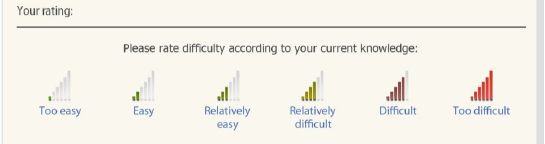
\includegraphics[width=\textwidth]{images/fig1.png}
\caption{Student rating estimation interface shown after interaction with exercise-type or question-type learning object.}
\label{fig1}
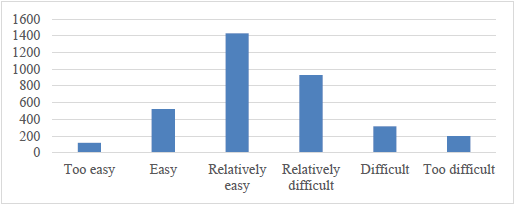
\includegraphics[width=0.95\textwidth]{images/fig2.png}
\caption{Observed student difficulty estimations for programming exercises over long term usage of ALEF.}
\label{fig2}
\end{figure}

We can, however, not only observe the ratings as aggregated per object averaging out ratings outside the ``real'' difficulty, but consider these individual ratings with the context of the user \textendash~specifically user knowledge during the rating \textendash~creating the dynamic difficulty estimation. We could then predict for a learner with similar knowledge that the given learning object is currently going to be too easy or too difficult for them and create recommendation list by selecting appropriate objects.

\section{Recommendation with dynamic student determined difficulty}
\label{sec3}

We propose a method for learning object recommendation based on the following assumptions from related work and observed user behaviour in ALEF:

%číselný zoznam
\begin{enumerate}
\item When a learner rates learning object difficulty, they consider not only objective general difficulty of the exercise/question, but they do so based on their experience with the learning object and their current knowledge.
\item An optimal learning object for the learner should have appropriate difficulty for their knowledge. If the learning object was too easy, both the learner would learn too little, and there would be little information gain for the user modelling component of the educational system. On the other hand, if the learning object was too difficult, the learner could be dissuaded from trying, or not even able to solve it.
\item Therefore, appropriate objects for a given learner are those, which they would, given their current knowledge, rate in the middle of the scale.
\end{enumerate}

The recommendation method looks for difficulty ratings of candidate learning objects (LOs) to be recommended. Only those ratings are considered, which are made by users who had the same or similar level of knowledge for relevant domain terms related to the given learning object during interaction with it and when expressing the difficulty rating afterwards. The method works as follows:

%prostredie pre zdrojový kód
\begin{verbatim}
function get_recommendations(user)
  var unsolved = find_unsolved_LOs(user, FADE_TIME)
  var lo_candidates = []

  foreach lo in unsolved
    difficulty = predicted_difficulty(user, lo)
    lo_candidates.add(lo, abs(difficulty - OPTIMAL_DIFF))
  end

  return lo_candidates.sort_by_difficulty.pick(TOP_N)
end
\end{verbatim}

We set optimal difficulty (\verb|OPTIMAL_DIFF|) to 0.5 from the range $\langle 0,1 \rangle$. Note that while we are looking for difficulty appropriate for the learner knowledge, which is not necessarily a difficulty 0.5 of the learning object, we are predicting difficulty from peer users considering their knowledge in the moment of rating, therefore this aspect is carried over in the predicted difficulty, not in the optimal difficulty. \verb|FADE_TIME| represents time function for which is the learning object considered solved and not to be recommended again. Its shape depends on how is the recommendation deployed, e.g., in long term use as a course support, a value related to (a multiple of) time distance between subsequent lessons should be used; in short term ``crash-courses'', the fade time can be in hours, or even infinite in order to not to repeat any learning objects at all. Here, we recommended top 4 items (\verb|TOP_N| = 4).

The difficulty predicted from similar peers is calculated as a weighted arithmetic mean of difficulty ratings from knowledge-similar users weighted by their similarity to target user (denoted \emph{U}):

%vzorec
$predicted\_difficulty (U,LO)$
$$=\frac{\sum_i rating (U_i, LO) * sim \Bigg(U, U_i, LO, time \Big(rating (U_i, LO)\Big)\Bigg)}{\sum_i sim (U, U_i, LO)}$$

The learner similarity for a given learning object considers only knowledge (understanding), \emph{underst(user, relevant\_term, time)}, of those relevant domain terms, \emph{prereq(LO)} that are required to understand and solve the given learning object, \emph{LO}. For a target user, we consider their current knowledge in the time of recommendation, and for peers, we consider their knowledge at the time when they produced rating for the object. The similarity is based on Euclidean distance of learners' knowledge:

%vzorec
$sim(U, U_x, LO, time) =$
$$1-\frac{\sqrt{\sum_{RDT_i\epsilon prereq(LO)}\Big(underst(U, RDT_i, now) - underst(U_x, RDT_i, time)\Big)^2}}{\sqrt{|prereq (LO)|}}$$

When the learner follows one of the shown recommendations and provides difficulty rating after the interaction, they form a feedback loop, both evaluating the recommendation and further contributing to the rating matrix for recommendation to other peers.

\section{Evaluation}
\label{sec4}

We evaluated the proposed method with students evenly distributed into two groups. One group was shown recommendations derived from learning object difficulty determined by peer students (the \emph{proposed method,} see section \ref{sec3}) and the other group was shown recommendations using static learning object difficulty estimated by a domain expert responsible for course authoring (a \emph{control method}).

The \emph{control method} gathers list of learning objects that could be possibly recommended (i.e., user has not solved them recently) and compares user's knowledge of all relevant domain terms that need to be understood to solve the exercise/question with its difficulty. For example, we are considering a learning object $LO_1$ to be recom-mended to user $U$ and in order to solve the $LO_1$, the user must have understood relevant domain terms $prereq(LO_1) = \{RDT_1 ...RDT_N\}$, e.g., in order to solve exercise $LO_1$= ``Number division'' (C programming language), relevant domain terms $RDT_1$= ``Operator \/'' and $RDT_2$ = ``double'' must be understood (multiple other terms are required, but omitted here for simplicity). If $underst(U, RDT_1) = 0.5$ and $underst(U, RDT_2) = 0.7$ and:

%vzorec
$$required\_knowledge(U, LO_1) = \frac{\sum_{RDT_i\epsilon prereq(LO_1)} underst(U, RDT_i)}{|prereq(LO_1)|}$$

then the required knowledge is in this case 0.6. This is compared with $difficulty (LO_1)$ and the closer is the user's knowledge to the difficulty, the more likely is $LO_1$ to be recommended. In other words, if the student knows very little from the prerequisites for a given learning object, the easier it must be in order to be appropriate to them, and vice versa, when the student knows almost everything needed for the learning object, it is only recommended when it is difficult, so it would still pose at least a little challenge to the student.

\emph{Results} We evaluated the proposed method in a controlled experiment with 30 students from various technical universities learning in the course on procedural programming using C language. The students have had some previous knowledge of procedural programming, some had experience specifically with the C language, therefore after a brief familiarization with the course by reading through some explanation-type learning objects, they were able to almost immediately start with both introductory and more advanced exercises and questions. Because the user input \textendash~difficulty rating after following a recommendation \textendash~is crucial for the proposed method to offer recommendation to other students, all students participated in the experiment at the same time in one three hour session.

Our hypotheses for the experiment were as follows:

%zoznam s odrážkami
\begin{itemize}
\item $H_1$. \emph{Learning objects recommended based on difficulty are more appropriate than those selected freely by students themselves.}
\item $H_2$. \emph{Learning objects recommended based on dynamic student determined difficulty (proposed method) are more appropriate than those recommended based on expert estimated static difficulty (control method).}
\item $H_3$. \emph{Students using appropriate learning objects recommended based on dynamic student determined difficulty do progress better during the learning session than control group.}
\end{itemize}

Originally, we expected to see differing levels of knowledge gained during the learning session (the strongest hypothesis $H_3$). However, the average knowledge achieved by students in the group $G_T$ with the proposed method was only slightly higher than the knowledge achieved in the control group $G_C$ (overall term knowledge of 13.6 \% as compared to 12.6 \%).

On the other hand, we evaluated the appropriateness of the recommended learning objects (hypotheses $H_1$ and $H_2$) by observing the difficulty ratings provided by the users after interacting with recommended items. To compare the recommendations based on difficulty (either made with the proposed method or the control method) against freely chosen learning objects ($H_1$), e.g., selected by browsing the menu, we looked at the properties of ratings observed in the experiment. The arithmetic mean of ratings was again 0.56 (the same as in long term usage without recommendation, see 3.1), however, the average expert estimated difficulty of the items was now 0.73. This suggest that while we recommended more difficult learning objects (speaking in terms of their static difficulty), they were appropriate for the learners given their knowledge, since they still rated them as medium difficulty (dynamic difficulty). The correlation with expert estimated static difficulty was also lower: $corr(x_u, x_e)$=0.53.

To compare the proposed and control method ($H_2$), we found the distance of individual difficulty ratings in the two groups from the target medium difficulty. In the proposed method, the distance was 20.0 \%, while in the control group, it was 31.6 \%. Using the dynamic student determined difficulty, we can make personalized recommendations of learning objects close to the optimal difficulty for the given learner.

\section{Rating quantity, rating elicitation and estimation}
\label{sec5}

In our experiment, participants were encouraged to rate learning object difficulty after interacting with an object. They actually provided these ratings very often, out of 796 visits to learning objects where difficulty is tracked (exercises and questions, but not explanations), there were 583 visits where the participant could rate difficulty (they attempted a solution, regardless of its correctness). Out of these, there were 532 ratings provided. 91.3 \% of the time when the participant was able to rate, they did.

In standard educational system usage this is, however, not the case. Out of 147,364 visits to exercises and questions in the ALEF system instance that is used in normal coursework, students have had the opportunity to rate difficulty in 48,820 cases, which is 33.1 \% of the visits. This ratio is sound due to the fact that when browsing for an exercise or question to try next, the student does not start interacting with all visited learning objects. Then, out of these, the rating was provided in 16,373 cases (34.3 \% times). The controlled recommendation experiment described in this paper was carried outside of this ALEF instance; visits and ratings during experiment do not contribute to these observations.

Approximately one in three times is still a relatively high visited-to-rated ratio compared to other domains, e.g. online stores, where items are browsed and/or bought many thousand times, but rated perhaps in hundreds of the cases. This can be explained from various reasons. A possible cause is the fact that students are informed by the ALEF that it personalizes their experience according to their inputs – and the ratings can be attributed to the following human motivations~\cite{9.}: when they perceive that they get better experience themselves – ``When I rate, I will get better recommen-dations.'', or when they perceive that they help others who might reciprocate – ``When I rate, I will inform others about too difficult or too easy exercises.''

The feedback quantity described above, when collected from many users, possibly over multiple iterations of the course in succeeding academic terms, can be enough for item recommendation. However, remind that our method performs filtering on the ratings by considering only ratings made by learners in the moment of their knowledge being similar to the target user. Therefore our target is to not only obtain as many ratings for learning objects as possible (have abundance of feedback), but to also cover various learner knowledge states, i.e. obtain difficulty ratings from as heterogeneous learners as possible and as often as possible. Ideally, each interaction with the learning object, regardless of its successfulness (learner has solved the execise/question correctly, incorrectly or even left it untouched), would end with learner rating its difficulty. We propose two approaches to either achieve or mimic this effect.

\emph{Adaptive explicit rating elicitation.} To further motivate the learners to provide ratings and also to collect the ratings in other key moments of interaction with the learning object, we can use an approach for adaptive explicit feedback elicitation, like the one we proposed for conversational evaluation of personalized approaches in~\cite{10.}. We conducted preliminary experiments, where we displayed modal (on top of the content) adaptive questions asking the user to rate learning object difficulty not only after the interaction is over, but while the learner is still solving the exercise or question.

When predicting whether a given item would be too difficult for a user, it is important to avoid so-called \emph{survivorship bias,} i.e. consider not only ratings of those who ``survived'' to the successful or unsuccessful end of interaction (providing correct or incorrect solution, or choosing that they do not know the solution), but also those, who may have left before. We asked users for their estimation of difficulty when they looked like they were leaving the exercise (e.g., started browsing the menu with the mouse cursor), or when they were partway through the interaction (e.g., they chose to see a hint for the exercise). While we may not be able to always exactly predict that the user is leaving, we can still obtain a difficulty rating. In the case when the learner persists afterwards, we can obtain another, final, rating for the given learning object. In the case when they leave, we have a rating from partial interaction, together with the information that the user did not finish or succeeded with such learning object and these can be valuable for more precise prediction of difficulty to others.

\emph{Estimating user perceived difficulty from implicit interactions.} Another option is to directly use information about user interaction with the learning object. Even when we do not obtain explicit rating from the user, in the future, we can consider implicit feedback suggesting that the item is too easy or too difficult, e.g., when the user starts solving, asks for hint, and then leaves, refusing or turning off adaptive questions. The time which it took for the learner to find the solution (normalized to personal speed of the learner), or number of retries in the programming exercises tested through solution-evaluator, are other possible candidates for difficulty estimation indicators.

\section{Conclusions}
\label{sec6}

In this paper, we centred on two approaches to learning object difficulty in adaptive educational systems: dynamic student determined difficulty and expert estimated static difficulty. The properties of these difficulty ratings were evaluated from the long term usage of ALEF adaptive educational system in multiple courses.

We proposed a recommendation method considering difficulty predicted for a given target user from difficulty ratings expressed by their peers while having similar knowledge to the target user. We also described a control recommendation method that picks learning object based only on knowledge of the target user and domain expert estimated difficulty. These two methods were compared in a controlled experiment with two groups of students using the proposed and the control method respectively. The group with proposed recommendation approach outperformed the control group only negligibly in the knowledge gained throughout the experiment, possibly due to the short scope of the experiment. However, the difficulty ratings expressed after using self-chosen learning objects and after using learning objects suggested by proposed and control methods suggest that the user learning experience is better using the difficulty-based recommendation method, since users receive learning objects with appropriate difficulty for them.

The control method which considered only user’s knowledge with static difficulty was afterwards deployed as a fall-back in \emph{cold-start} scenarios, when the learner has not yet made enough actions to estimate their knowledge and find similar users, or when there are insufficient peer difficulty ratings to recommend learning objects.

In future work, the recommendation can be further personalized for preferences of each learner. We have assumed that the optimal exercises/questions are those with medium difficulty for the learner’s current knowledge, which is actually best to progress further without dissuading the learner and to model user's knowledge. However one learner can welcome the challenge and prefer more difficult learning objects, or on the other hand can be easily dissuaded by even moderately difficult ones. This could be detected, for example, by comparing learner ratings after using recommendations to their peer ratings, by observing successfulness of solving recommended items, or even by observing whether the learner has left the learning object without attempting a solution. Conserving the same rating prediction mechanisms described here, one learner could receive recommendations computed for different (personalized) target difficulty than another.

%acknowledgement
\textbf\ackname This work was partially supported by grants. No. VG1/0971/11,KEGA 009STU-4/2014, and APVV-0233-10. We thank Matej Noga for recommend-er method implementation in ALEF system.

%referencie
\bibliographystyle{splncs03}
\bibliography{zdroje}





















\end{document}